% Section: Simulation environment and turbine model
\section{Simulation environment and turbine model}
\label{sec:methods}

% TODO: Step E0: frozen environment (OpenFAST v4.2.1, r-test, binaries, MATLAB R2024a, machine); single-precision OpenFAST build to be declared.
\subsection{Aerodynamic model and its verification}
\label{subsec:aero_verification}
{\color{revQ1}
The plant is the land-based NREL 5-MW reference wind turbine~\cite{jonkman2009}, simulated with OpenFAST v4.2.1 (ElastoDyn structural model, AeroDyn blade-element momentum aerodynamics, ServoDyn control interface) using the input files of the OpenFAST regression-test suite. Before any controller is designed, the aerodynamic model is checked against the values published by Jonkman \emph{et al.}~\cite{jonkman2009}, with acceptance criteria fixed before the computations. Three steady-state sweeps were computed with the OpenFAST aerodynamic-map solver: (i) at a fixed wind speed of 8~m/s, varying rotor speed and collective pitch, as in~\cite{jonkman2009}; (ii) at the rated rotor speed of 12.1~rpm, for the fifteen wind speeds of~\cite[Table~7-1]{jonkman2009}; (iii) on a tip-speed-ratio and pitch grid at 12.1~rpm, which provides the $C_p(\lambda,\beta)$ table used by the physics-based internal model.

Figure~\ref{fig:E1_peak} shows the power coefficient computed near its maximum at a fixed wind speed of 8~m/s, for collective pitch angles around zero, together with the peak reported in~\cite{jonkman2009}. The computed peak is 0.4825 at $\lambda = 7.50$ and $\beta = -0.25^\circ$ (grid values), against 0.482 at $\lambda = 7.55$ and $\beta = 0^\circ$ reported in~\cite{jonkman2009}. Figure~\ref{fig:E1_beq} compares, above rated wind speed, the equilibrium pitch angles that hold the aerodynamic power at the rated mechanical power of 5.296610~MW~\cite{jonkman2009} with the values of~\cite[Table~7-1]{jonkman2009} (top panel), and shows their difference (bottom panel); over the fifteen wind speeds from 11.4 to 25~m/s, the maximum deviation is $0.33^\circ$ (at 25~m/s). The pitch sensitivities $\partial P/\partial\theta$ obtained from these steady-state equilibria are between 0.11 (at 11.4~m/s, where the equilibrium pitch is saturated at $0^\circ$) and 0.87 times the published values; since the latter were obtained by a frozen-wake linearization~\cite{jonkman2009}, the two quantities are compared indicatively only.
}

\begin{figure}[htbp]
\centering
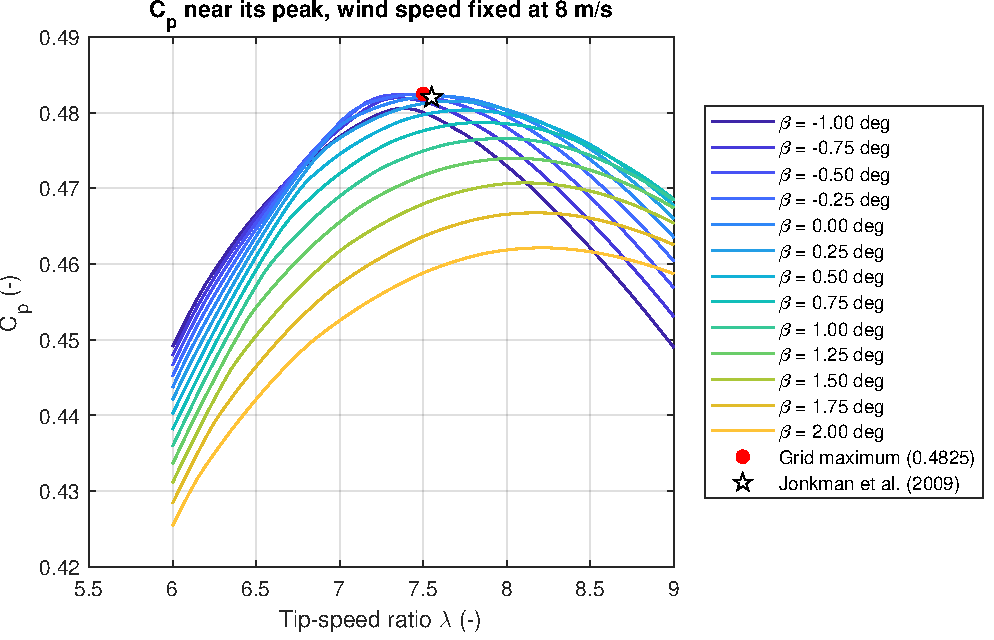
\includegraphics[width=0.8\linewidth]{figures/E1_fig3_Cp_peak_region.pdf}
\caption{{\color{revQ1}Power coefficient near its maximum at a fixed wind speed of 8~m/s, for collective pitch angles around zero (OpenFAST aerodynamic-map solver, converged points only). Filled circle: computed grid maximum; star: value reported in~\cite{jonkman2009}.}}
\label{fig:E1_peak}
\end{figure}

\begin{figure}[htbp]
\centering
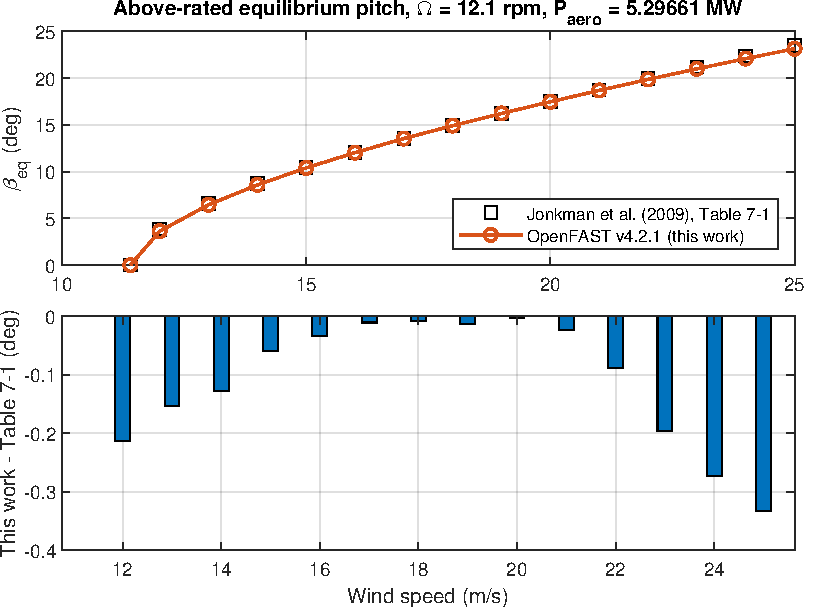
\includegraphics[width=0.8\linewidth]{figures/E1_fig2_equilibrium_pitch_vs_wind.pdf}
\caption{{\color{revQ1}Top: equilibrium collective pitch at the rated rotor speed and rated mechanical power, computed with OpenFAST (circles) and reported in~\cite[Table~7-1]{jonkman2009} (squares). Bottom: difference between the two (this work minus Table~7-1).}}
\label{fig:E1_beq}
\end{figure}
\subsection{Reduced-order physics model}
\label{subsec:rom}
{\color{revQ1}
The internal model of the physics-based NMPC is a two-state reduced-order model of the same turbine. Its states are the rotor speed $\omega_r$ and the filtered generator speed $\omega_f$, obtained with the first-order low-pass filter of corner frequency 0.25~Hz used by the baseline controller~\cite{jonkman2009}. The rotor speed obeys a single-rigid-mass drivetrain equation, $J\,\dot{\omega}_r = Q_\mathrm{aero} - N\,Q_g$, where $J$ is the rotor inertia including the generator inertia referred to the low-speed shaft and $N$ is the gearbox ratio. The aerodynamic torque is $Q_\mathrm{aero} = \tfrac{1}{2}\rho\pi R^3 V^2 C_p(\lambda,\beta)/\lambda$, with $\lambda = \omega_r R/V$, where $C_p(\lambda,\beta)$ is interpolated, without extrapolation, in the table of sweep (iii) of Section~\ref{subsec:aero_verification}. The generator torque $Q_g$ follows the baseline variable-speed torque law of~\cite{jonkman2009}, evaluated on $\omega_f$ and on the collective pitch angle $\beta$, which is the manipulated variable and has no actuator dynamics in the model. The model is discretized with a sample time of 0.05~s by a fourth-order Runge--Kutta scheme with four sub-steps. Its declared simplifications are a rigid drivetrain, no mechanical loss term, quasi-steady aerodynamics and the absence of a torque-rate limit.

The model was compared with the OpenFAST plant in closed loop with the baseline controller of~\cite{jonkman2009} (Section~\ref{sec:reference}), on 21 turbulent runs at seven mean wind speeds from 12 to 24~m/s, with three turbulence seeds per speed. From $t = 60$~s, each run is cut into consecutive segments of 1.5~s, the prediction horizon of the NMPC. At the start of each segment the model is reinitialized on the OpenFAST rotor speed; it is then driven by the recorded pitch angle and wind input, each held over one sample time, and its rotor speed is compared with that of OpenFAST. The acceptance criterion, fixed before the computations, requires at each mean wind speed a median of the maximum absolute rotor-speed error $e_{\max}$ over the segments of at most 2\,\% of the rated rotor speed, and a 95th percentile (P95) of at most 5\,\%; segments in which the model leaves the domain of the $C_p$ table count as failures. With the wind speed at hub height as wind input (model v1), the criterion was not met at any mean wind speed: the median of $e_{\max}$ ranged from 2.36 to 4.28\,\% and its P95 from 7.30 to 11.23\,\% of the rated rotor speed.

After an exploratory diagnostic on these runs, the wind input was replaced by the rotor-effective wind speed computed by AeroDyn, namely the axial component, in hub axes, of the inflow velocity averaged over all blade nodes minus the blade elastic velocity (model v2); the equations, parameters and $C_p$ table are unchanged. This signal is not measurable on a real turbine: it is assumed perfectly known by every controller compared in this paper, which is an idealization. Because this input was chosen after examining the first turbulent runs, model v2 was tested on 21 new runs with three new turbulence seeds, with the same segments, protocol and criterion. Figure~\ref{fig:E2_emax} shows, at each mean wind speed, the median and the P95 of $e_{\max}$ for both models, together with the two thresholds. Model v2 met the criterion at all seven mean wind speeds: the median of $e_{\max}$ ranged from 0.56 to 1.25\,\% and its P95 from 1.54 to 2.73\,\% of the rated rotor speed. Model v2 was also replayed on six runs in steady wind at 14, 18 and 22~m/s, in which the collective pitch angle is driven from $t = 60$~s, at a rate of 8~$^\circ$/s, to the equilibrium pitch angle of Section~\ref{subsec:aero_verification} plus or minus $1^\circ$; since the pitch angle at $t = 60$~s is not exactly at this equilibrium value, the realized pitch changes differ from $\pm 1^\circ$. The largest $e_{\max}$ over the first 1.5~s was 0.65\,\% of the rated rotor speed, for a criterion of 2\,\%.
}

\begin{figure}[htbp]
\centering
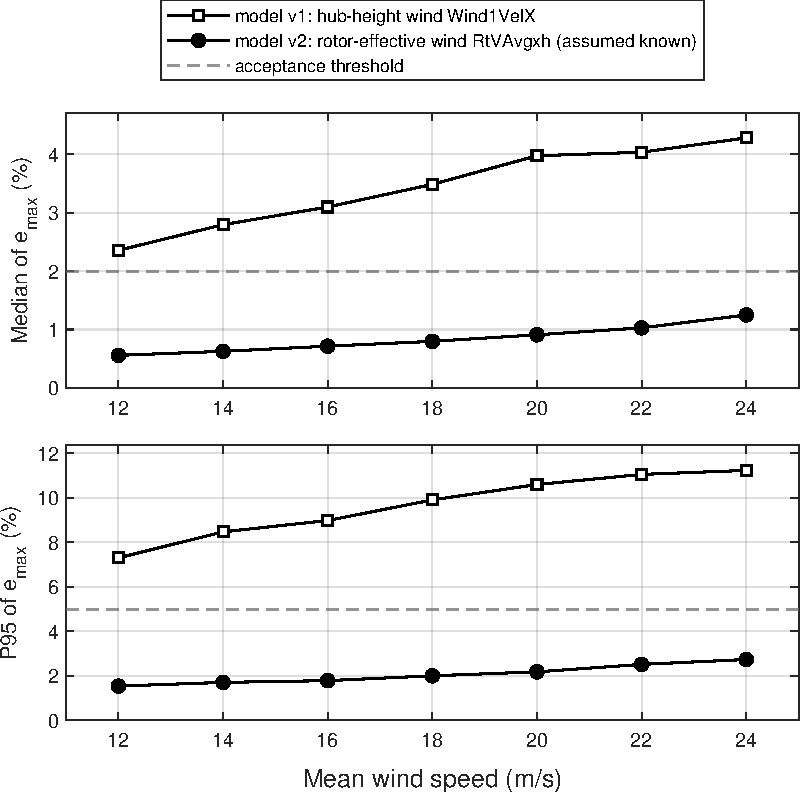
\includegraphics[width=0.8\linewidth]{figures/E2_fig1_emax_by_speed.pdf}
\caption{{\color{revQ1}Median (top) and 95th percentile (bottom) of the maximum absolute rotor-speed error $e_{\max}$ of the reduced-order model over 1.5-s segments of turbulent closed-loop OpenFAST runs, in percent of the rated rotor speed, at each mean wind speed (three seeds pooled). Squares: model v1, driven by the hub-height wind speed (first set of runs); circles: model v2, driven by the rotor-effective wind speed assumed known (new seeds). Dashed lines: acceptance thresholds (2\,\% and 5\,\%).}}
\label{fig:E2_emax}
\end{figure}
